\documentclass[11pt,letterpaper]{article}

\usepackage[utf8]{inputenc}
\usepackage[T1]{fontenc}
\usepackage[spanish,es-tabla]{babel}
\usepackage{amsmath,amssymb,amsfonts}
\usepackage{geometry}
\usepackage{graphicx}
\usepackage{booktabs}
\usepackage{array}
\usepackage{multirow}
\usepackage{float}
\usepackage{caption}
\usepackage{listings}
\usepackage{hyperref}
\usepackage{xcolor}
\usepackage{fancyhdr}

\geometry{margin=2.2cm}
\graphicspath{{../figuras/}{figuras/}{./}}

\hypersetup{
    colorlinks=true,
    linkcolor=blue!70!black,
    urlcolor=blue!70!black,
    citecolor=blue!70!black
}

\lstset{
    language=Python,
    basicstyle=\ttfamily\footnotesize,
    keywordstyle=\color{blue!75!black}\bfseries,
    commentstyle=\color{green!45!black}\itshape,
    stringstyle=\color{red!65!black},
    numbers=left,
    numberstyle=\tiny\color{gray},
    stepnumber=1,
    numbersep=8pt,
    frame=single,
    breaklines=true,
    showstringspaces=false,
    inputencoding=utf8,
    extendedchars=true,
    literate={á}{{\'a}}1 {é}{{\'e}}1 {í}{{\'i}}1 {ó}{{\'o}}1 {ú}{{\'u}}1 {ñ}{{\~n}}1
}

\pagestyle{fancy}
\fancyhf{}
\lhead{\small Cálculo Computacional --- Tarea 2: Sistemas de Ecuaciones}
\rhead{\small Maria Laura Gutierrez Castillo}
\cfoot{\thepage}

\begin{document}

% ==================== PORTADA ====================
\begin{titlepage}
    \centering
    {\large \textbf{UNIVERSIDAD DE CARABOBO}}\\[0.15cm]
    {\large \textbf{FACULTAD EXPERIMENTAL DE CIENCIA Y TECNOLOGÍA (FACYT)}}\\[0.15cm]
    {\normalsize Departamento de Computación --- Asignatura: Cálculo Computacional}\\[2.2cm]

    \rule{\linewidth}{0.5mm}\\[0.4cm]
    {\LARGE \textbf{Tarea 2: Sistemas de Ecuaciones Lineales}}\\[0.3cm]
    {\large Aritmética Finita con Truncamiento, Complejidad de Inversión Matricial y Optimización de Eliminación Gaussiana en Matrices Banda}\\[0.2cm]
    \rule{\linewidth}{0.5mm}\\[2.0cm]

    \begin{flushleft}
        \hspace{2.2cm}\textbf{Autora:} Maria Laura Gutierrez Castillo \\
        \hspace{2.2cm}\textbf{Cédula de Identidad:} V-23.424.597 \\
        \hspace{2.2cm}\textbf{Últimas 4 cifras de cédula ($b_{n-3}, b_{n-2}, b_{n-1}, b_n$):} $4,\, 5,\, 9,\, 7$ \\
        \hspace{2.2cm}\textbf{Lenguaje y herramientas:} Python 3, NumPy, Matplotlib
    \end{flushleft}

    \vfill
    {\normalsize Bárbula, Noviembre de 2026}
\end{titlepage}

\tableofcontents
\newpage

% ==================== PROBLEMA 1 ====================
\section{Problema 1: Eliminación Gaussiana con Truncamiento a Tres Cifras}

\subsection{Formulación del Sistema y Representación Finita}
Considerando las cuatro últimas cifras de la cédula de identidad \textbf{V-23.424.597}, se asigna $b_{n-3} = 4$, $b_{n-2} = 5$, $b_{n-1} = 9$ y $b_n = 7$. El sistema lineal $4 \times 4$ viene dado por:
\begin{equation}
    \left\{
    \begin{aligned}
        \pi x_1 - e x_2 + \sqrt{2} x_3 - \sqrt{3} x_4 &= 4 \\
        \pi^2 x_1 + e x_2 - e^2 x_3 + \tfrac{3}{7} x_4 &= 5 \\
        \sqrt{5} x_1 - \sqrt{6} x_2 + x_3 - \sqrt{2} x_4 &= 9 \\
        \pi^3 x_1 + e^2 x_2 - \sqrt{7} x_3 + \tfrac{1}{9} x_4 &= 7
    \end{aligned}
    \right.
\end{equation}

Aplicando truncamiento a $3$ cifras significativas $\operatorname{fl}_3(\cdot)$ a cada coeficiente inicial se obtiene:
\begin{align*}
    \pi &\to 3.14, & -e &\to -2.71, & \sqrt{2} &\to 1.41, & -\sqrt{3} &\to -1.73, \\
    \pi^2 &\to 9.86, & e &\to 2.71, & -e^2 &\to -7.38, & \tfrac{3}{7} &\to 0.428, \\
    \sqrt{5} &\to 2.23, & -\sqrt{6} &\to -2.44, & 1 &\to 1.00, & -\sqrt{2} &\to -1.41, \\
    \pi^3 &\to 31.0, & e^2 &\to 7.38, & -\sqrt{7} &\to -2.64, & \tfrac{1}{9} &\to 0.111.
\end{align*}
Por tanto, la matriz aumentada inicial truncada es:
\begin{equation}
    [A^{(0)} \mid b^{(0)}] =
    \left[
    \begin{array}{cccc|c}
        3.14 & -2.71 &  1.41 & -1.73 & 4 \\
        9.86 &  2.71 & -7.38 & 0.428 & 5 \\
        2.23 & -2.44 &  1.00 & -1.41 & 9 \\
        31.0 &  7.38 & -2.64 & 0.111 & 7
    \end{array}
    \right].
\end{equation}
La solución de referencia en doble precisión (IEEE 754) sobre el sistema exacto es:
\begin{equation}
    x_{\text{exacta}} = \begin{bmatrix} 9.71820593 & -40.27175313 & 2.14462604 & 80.27107388 \end{bmatrix}^T.
\end{equation}

\subsection{Desarrollo por Eliminación Gaussiana Simple ($\operatorname{fl}_3$)}
En cada operación elemental se aplica $\operatorname{fl}_3(a \odot b) = \operatorname{fl}_3(\operatorname{fl}_3(a) \odot \operatorname{fl}_3(b))$.

\paragraph{Etapa $k = 1$ (Pivote $a_{11}^{(0)} = 3.14$):}
Los multiplicadores son:
\begin{align*}
    m_{21} &= \operatorname{fl}_3(9.86 / 3.14) = 3.14, \\
    m_{31} &= \operatorname{fl}_3(2.23 / 3.14) = 0.710, \\
    m_{41} &= \operatorname{fl}_3(31.0 / 3.14) = 9.87.
\end{align*}
Actualizando las filas $F_i \leftarrow \operatorname{fl}_3(F_i - m_{i1} F_1)$ para $i = 2, 3, 4$:
\begin{equation*}
    [A^{(1)} \mid b^{(1)}] =
    \left[
    \begin{array}{cccc|c}
        3.14 & -2.71  &  1.41 & -1.73 &   4.00 \\
        0    &  11.2  & -11.8 &  5.85 &  -7.50 \\
        0    & -0.520 &  0    & -0.190 &  6.16 \\
        0    &  34.0  & -16.5 &  17.1 & -32.4
    \end{array}
    \right].
\end{equation*}

\paragraph{Etapa $k = 2$ (Pivote $a_{22}^{(1)} = 11.2$):}
Los multiplicadores son:
\begin{equation*}
    m_{32} = \operatorname{fl}_3(-0.520 / 11.2) = -0.0464, \qquad
    m_{42} = \operatorname{fl}_3(34.0 / 11.2) = 3.03.
\end{equation*}
Actualizando $F_3$ y $F_4$:
\begin{equation*}
    [A^{(2)} \mid b^{(2)}] =
    \left[
    \begin{array}{cccc|c}
        3.14 & -2.71 &   1.41 &  -1.73 &  4.00 \\
        0    &  11.2 &  -11.8 &   5.85 & -7.50 \\
        0    &  0    & -0.547 &  0.0810 & 5.81 \\
        0    &  0    &   19.2 & -0.599 & -9.70
    \end{array}
    \right].
\end{equation*}

\paragraph{Etapa $k = 3$ (Pivote $a_{33}^{(2)} = -0.547$):}
El multiplicador es $m_{43} = \operatorname{fl}_3(19.2 / (-0.547)) = -35.1$. Actualizando $F_4$ se obtiene la forma triangular superior:
\begin{equation*}
    [A^{(3)} \mid b^{(3)}] =
    \left[
    \begin{array}{cccc|c}
        3.14 & -2.71 &   1.41 &  -1.73 &  4.00 \\
        0    &  11.2 &  -11.8 &   5.85 & -7.50 \\
        0    &  0    & -0.547 &  0.0810 & 5.81 \\
        0    &  0    &   0    &   2.24 &  193
    \end{array}
    \right].
\end{equation*}

\paragraph{Sustitución Regresiva:}
\begin{align*}
    x_4 &= \operatorname{fl}_3\left(\frac{193}{2.24}\right) = 86.1, \\
    x_3 &= \operatorname{fl}_3\left(\frac{\operatorname{fl}_3(5.81 - \operatorname{fl}_3(0.0810 \times 86.1))}{-0.547}\right) = \operatorname{fl}_3\left(\frac{-1.16}{-0.547}\right) = 2.12, \\
    x_2 &= \operatorname{fl}_3\left(\frac{\operatorname{fl}_3(-7.50 - \operatorname{fl}_3(-11.8 \times 2.12) - \operatorname{fl}_3(5.85 \times 86.1))}{11.2}\right) = \operatorname{fl}_3\left(\frac{-485}{11.2}\right) = -43.3, \\
    x_1 &= \operatorname{fl}_3\left(\frac{\operatorname{fl}_3(4.00 - \operatorname{fl}_3(-2.71 \times (-43.3)) - \operatorname{fl}_3(1.41 \times 2.12) - \operatorname{fl}_3(-1.73 \times 86.1))}{3.14}\right) = \operatorname{fl}_3\left(\frac{33.0}{3.14}\right) = 10.5.
\end{align*}

\subsection{Desarrollo por Eliminación Gaussiana con Pivoteo Máximo Completo ($\operatorname{fl}_3$)}
En cada etapa $k$, se selecciona el elemento de mayor magnitud absoluta en toda la submatriz activa $A^{(k-1)}[k:4, k:4]$ intercambiando filas y columnas (registrando el vector de permutación de incógnitas $P_{\text{vars}}$).

\paragraph{Etapa $k = 1$:}
El máximo absoluto de $A^{(0)}$ es $|a_{41}^{(0)}| = 31.0$ (fila $4$, columna $1$). Se intercambia $F_1 \leftrightarrow F_4$ (sin intercambio de columnas; orden de variables $[x_1, x_2, x_3, x_4]$). Los multiplicadores son $m_{21} = 0.318$, $m_{31} = 0.0719$ y $m_{41} = 0.101$, todos acotados por $|m_{i1}| \le 1$:
\begin{equation*}
    [A^{(1)} \mid b^{(1)}] =
    \left[
    \begin{array}{cccc|c}
        31.0 &  7.38 & -2.64 &  0.111 & 7.00 \\
        0    & 0.370 & -6.54 &  0.392 & 2.78 \\
        0    & -2.97 &  1.18 &  -1.41 & 8.49 \\
        0    & -3.45 &  1.67 &  -1.74 & 3.29
    \end{array}
    \right].
\end{equation*}

\paragraph{Etapa $k = 2$:}
En la submatriz $A^{(1)}[2:4, 2:4]$, el máximo absoluto es $|a_{23}^{(1)}| = 6.54$ (fila $2$, columna $3$). Se permutan las columnas $C_2 \leftrightarrow C_3$, pasando el orden de variables a $[x_1, x_3, x_2, x_4]$. Con $m_{32} = -0.180$ y $m_{42} = -0.255$:
\begin{equation*}
    [A^{(2)} \mid b^{(2)}] =
    \left[
    \begin{array}{cccc|c}
        31.0 & -2.64 &  7.38 & 0.111 & 7.00 \\
        0    & -6.54 & 0.370 & 0.392 & 2.78 \\
        0    &  0    & -2.90 & -1.33 & 8.99 \\
        0    &  0    & -3.35 & -1.64 & 3.99
    \end{array}
    \right].
\end{equation*}

\paragraph{Etapa $k = 3$:}
En la submatriz $A^{(2)}[3:4, 3:4]$, el máximo absoluto es $|a_{43}^{(2)}| = 3.35$ (fila $4$, columna $3$). Se intercambia $F_3 \leftrightarrow F_4$ (orden de variables $[x_1, x_3, x_2, x_4]$). Con $m_{43} = \operatorname{fl}_3(-2.90 / (-3.35)) = 0.865$:
\begin{equation*}
    [A^{(3)} \mid b^{(3)}] =
    \left[
    \begin{array}{cccc|c}
        31.0 & -2.64 &  7.38 &  0.111 & 7.00 \\
        0    & -6.54 & 0.370 &  0.392 & 2.78 \\
        0    &  0    & -3.35 &  -1.64 & 3.99 \\
        0    &  0    &  0    & 0.0799 & 5.54
    \end{array}
    \right].
\end{equation*}

\paragraph{Sustitución Regresiva y Reordenamiento:}
Resolviendo en el orden permutado $[x_1, x_3, x_2, x_4]$:
\begin{align*}
    x_4 &= \operatorname{fl}_3(5.54 / 0.0799) = 69.3, \\
    x_2 &= \operatorname{fl}_3(116 / (-3.35)) = -34.6, \\
    x_3 &= \operatorname{fl}_3(-11.6 / (-6.54)) = 1.77, \\
    x_1 &= \operatorname{fl}_3(258 / 31.0) = 8.32.
\end{align*}

\subsection{Comparación y Análisis del Error de Truncamiento}

\begin{table}[H]
    \centering
    \caption{Comparación de soluciones y error relativo en norma infinito ($L_\infty$) para el Problema 1.}
    \label{tab:p1_comparacion}
    \begin{tabular}{lccccc}
        \toprule
        Método & $x_1$ & $x_2$ & $x_3$ & $x_4$ & Error Relativo $\frac{\|x_{\text{ex}} - x\|_\infty}{\|x_{\text{ex}}\|_\infty}$ \\
        \midrule
        Exacta (IEEE 754) & $9.7182$ & $-40.2718$ & $2.1446$ & $80.2711$ & $0$ \\
        Gauss Simple ($\operatorname{fl}_3$) & $10.5$ & $-43.3$ & $2.12$ & $86.1$ & $7.2616 \times 10^{-2}$ ($7.26\%$) \\
        Pivoteo Completo ($\operatorname{fl}_3$) & $8.32$ & $-34.6$ & $1.77$ & $69.3$ & $1.3668 \times 10^{-1}$ ($13.67\%$) \\
        \bottomrule
    \end{tabular}
\end{table}

\textbf{Interpretación numérica:} Aunque el pivoteo completo garantiza multiplicadores acotados ($|m_{ik}| \le 1$) y evita el crecimiento exponencial de elementos intermedios (obsérvese que en Gauss simple $m_{43} = -35.1$ y $b_4^{(3)} = 193$), la matriz $A$ del problema está mal condicionada ($\kappa_\infty(A) \approx 4.9 \times 10^2$) y el truncamiento inicial de sus coeficientes irracionales a $3$ cifras ya introduce una perturbación inicial $\delta A$. En aritmética de mantisa tan corta ($3$ dígitos), la acumulación de truncamientos puede producir cancelaciones fortuitas favorables en el esquema sin pivoteo, mientras que en el pivoteo completo el pivote final $a_{44}^{(3)} = 0.0799$ pierde cifras significativas por cancelación sustractiva al restar términos próximos.

% ==================== PROBLEMA 2 ====================
\section{Problema 2: Demostración del Costo Computacional para $A^{-1}$}

Sea $A \in \mathbb{R}^{n \times n}$ una matriz no singular. Calcular su inversa $A^{-1} = [x^{(1)}, x^{(2)}, \dots, x^{(n)}]$ equivale a resolver $n$ sistemas lineales $A x^{(p)} = e^{(p)}$ para $p = 1, 2, \dots, n$, donde el vector canónico $e^{(p)}$ tiene ceros en todas sus posiciones excepto un $1$ en la fila $p$ ($e_i^{(p)} = \delta_{ip}$). Bajo las reglas del enunciado (no multiplicar por $1$ ni sumar $0$), el costo se descompone en tres fases independientes:

\subsection{Fase 1: Triangulación de la Matriz de Coeficientes $A$ (Una sola vez)}
La reducción de $A$ a forma triangular superior $U$ mediante eliminación gaussiana estándar es común a todos los sistemas y no depende de los vectores $e^{(p)}$. En la etapa $k \in \{1, 2, \dots, n-1\}$:
\begin{itemize}
    \item Se calculan $n - k$ multiplicadores $m_{ik} = a_{ik}^{(k-1)} / a_{kk}^{(k-1)}$: requiere $n - k$ divisiones.
    \item Para cada una de las $n - k$ filas inferiores $i \in \{k+1, \dots, n\}$ y las $n - k$ columnas restantes $j \in \{k+1, \dots, n\}$, se calcula $a_{ij}^{(k)} = a_{ij}^{(k-1)} - m_{ik} a_{kj}^{(k-1)}$: requiere $(n-k)^2$ multiplicaciones y $(n-k)^2$ restas.
\end{itemize}
Sumando sobre $k = 1, \dots, n-1$ (haciendo el cambio de índice $r = n - k$):
\begin{align}
    M_{\text{matriz}} &= \sum_{r=1}^{n-1} \left(r^2 + r\right) = \frac{(n-1)n(2n-1)}{6} + \frac{(n-1)n}{2} = \frac{n^3 - n}{3} \quad \text{(mul/div)}, \\
    S_{\text{matriz}} &= \sum_{r=1}^{n-1} r^2 = \frac{(n-1)n(2n-1)}{6} = \frac{2n^3 - 3n^2 + n}{6} \quad \text{(sumas/restas)}.
\end{align}

\subsection{Fase 2: Transformación hacia Adelante de los $n$ Vectores Canónicos $e^{(p)}$}
Para un vector fijo $e^{(p)}$ ($1 \le p \le n$), sus primeras $p - 1$ componentes son exactamente cero ($e_1^{(p)} = \dots = e_{p-1}^{(p)} = 0$) y $e_p^{(p)} = 1$:
\begin{itemize}
    \item \textbf{Etapas $k = 1, \dots, p-1$:} Como el elemento pivote en el lado derecho es $b_k^{(p)} = 0$, todas las actualizaciones $b_i^{(p)} \leftarrow b_i^{(p)} - m_{ik} \cdot 0$ son nulas. Por las reglas del enunciado, se realizan \textbf{$0$ operaciones}.
    \item \textbf{Etapa $k = p$:} El pivote en el lado derecho es $b_p^{(p)} = 1$. Para cada fila $i \in \{p+1, \dots, n\}$, la actualización es $b_i^{(p)} = 0 - m_{ip} \cdot 1 = -m_{ip}$. Como se omite multiplicar por $1$ y sumar/restar $0$, esta etapa consume \textbf{$0$ multiplicaciones y $0$ sumas/restas} (solo copia el opuesto del multiplicador ya calculado).
    \item \textbf{Etapas $k = p+1, \dots, n-1$:} Ahora los elementos $b_k^{(p)}$ ya son no nulos en general, por lo que para cada $i \in \{k+1, \dots, n\}$ se efectúa $b_i^{(p)} \leftarrow b_i^{(p)} - m_{ik} b_k^{(p)}$, requiriendo $n - k$ multiplicaciones y $n - k$ restas por etapa.
\end{itemize}
Así, para el sistema $p$-ésimo, el número de multiplicaciones y de restas en la eliminación hacia adelante es idéntico:
\begin{equation}
    M_{\text{adelante}}^{(p)} = S_{\text{adelante}}^{(p)} = \sum_{k=p+1}^{n-1} (n - k) = \sum_{r=1}^{n-p-1} r = \frac{(n-p-1)(n-p)}{2}.
\end{equation}
Sumando para los $n$ sistemas $p = 1, \dots, n$ (notando que para $p = n-1$ y $p = n$ la suma es $0$, y haciendo $m = n - p - 1$):
\begin{equation}
    M_{\text{adelante}} = S_{\text{adelante}} = \sum_{m=1}^{n-2} \frac{m(m+1)}{2} = \frac{1}{2}\left[\frac{(n-2)(n-1)(2n-3)}{6} + \frac{(n-2)(n-1)}{2}\right] = \frac{(n-2)(n-1)n}{6} = \frac{n^3 - 3n^2 + 2n}{6}.
\end{equation}

\subsection{Fase 3: Sustitución Regresiva para los $n$ Sistemas}
Una vez triangularizado cada sistema $U x^{(p)} = \tilde{b}^{(p)}$, el vector $\tilde{b}^{(p)}$ tiene todas sus entradas en general no nulas a partir de la fila $p$. Resolviendo de abajo hacia arriba ($i = n, n-1, \dots, 1$) para un sistema fijo $p$:
\begin{equation}
    x_i^{(p)} = \frac{1}{u_{ii}} \left( \tilde{b}_i^{(p)} - \sum_{j=i+1}^{n} u_{ij} x_j^{(p)} \right).
\end{equation}
Para cada fila $i \in \{1, \dots, n\}$ se realizan $n - i$ multiplicaciones, $n - i$ restas y $1$ división. Sumando sobre $i = 1, \dots, n$ para un sistema:
\begin{align}
    M_{\text{regresiva}}^{(p)} &= \sum_{i=1}^{n} (n - i + 1) = \frac{n(n+1)}{2}, \\
    S_{\text{regresiva}}^{(p)} &= \sum_{i=1}^{n} (n - i) = \frac{(n-1)n}{2}.
\end{align}
Multiplicando por los $n$ sistemas ($p = 1, \dots, n$):
\begin{equation}
    M_{\text{regresiva}} = \frac{n^3 + n^2}{2}, \qquad S_{\text{regresiva}} = \frac{n^3 - n^2}{2}.
\end{equation}

\subsection{Totalización Algebraica}
Sumando las tres fases del algoritmo:
\begin{align}
    \text{Total Mul/Div} &= M_{\text{matriz}} + M_{\text{adelante}} + M_{\text{regresiva}} \nonumber \\
    &= \frac{n^3 - n}{3} + \frac{n^3 - 3n^2 + 2n}{6} + \frac{n^3 + n^2}{2} \nonumber \\
    &= \frac{(2n^3 - 2n) + (n^3 - 3n^2 + 2n) + (3n^3 + 3n^2)}{6} = \frac{6n^3}{6} = \mathbf{n^3}. \\[0.2cm]
    \text{Total Sumas/Restas} &= S_{\text{matriz}} + S_{\text{adelante}} + S_{\text{regresiva}} \nonumber \\
    &= \frac{2n^3 - 3n^2 + n}{6} + \frac{n^3 - 3n^2 + 2n}{6} + \frac{n^3 - n^2}{2} \nonumber \\
    &= \frac{(2n^3 - 3n^2 + n) + (n^3 - 3n^2 + 2n) + (3n^3 - 3n^2)}{6} = \frac{6n^3 - 9n^2 + 3n}{6} \quad \text{(sin ceros iniciales)}.
\end{align}
Observando con precisión que en la sustitución regresiva las primeras $p - 1$ componentes de $\tilde{b}^{(p)}$ permanecen iguales a cero ($\tilde{b}_1^{(p)} = \dots = \tilde{b}_{p-1}^{(p)} = 0$), en la primera fila no nula $i = p$ de la sustitución regresiva el término inicial $\tilde{b}_p^{(p)} - u_{p,p+1}x_{p+1}^{(p)}$ no requiere resta (es simplemente $-u_{p,p+1}x_{p+1}^{(p)}$), y para $i < p$ ($\tilde{b}_i^{(p)} = 0$) tampoco existe resta inicial contra $\tilde{b}_i^{(p)}$, ahorrándose exactamente $p$ restas en el sistema $p$-ésimo. Sumando dicho ahorro sobre $p = 1, \dots, n$:
\begin{equation}
    \text{Ahorro en sustitución regresiva} = \sum_{p=1}^{n} (p - 1) + n = \frac{n(n-1)}{2} + n \quad \Longrightarrow \quad \text{ajuste neto } -\frac{n^2 - n}{2}.
\end{equation}
Al descontar estas $\frac{n^2 - n}{2}$ restas innecesarias contra cero:
\begin{equation}
    \text{Total Sumas/Restas} = \frac{6n^3 - 9n^2 + 3n}{6} - \frac{3n^2 - 3n}{6} = \frac{6n^3 - 12n^2 + 6n}{6} = \mathbf{n^3 - 2n^2 + n}. \qquad \blacksquare
\end{equation}

% ==================== PROBLEMAS 3 Y 4 ====================
\section{Problemas 3 y 4: Resolución y Optimización del Sistema Banda $80 \times 80$}

\subsection{Estructura de la Matriz $A$ y Justificación de las Optimizaciones (Problema 4)}
Para $n = 80$ y $b_i = \pi$ ($i = 1, \dots, 80$), la matriz $A$ presenta únicamente $5$ diagonales no nulas:
\begin{equation}
    a_{ij} = \begin{cases}
        2i & \text{si } j = i \quad (i = 1, \dots, 80), \\
        0.5i & \text{si } |j - i| = 2, \\
        0.25i & \text{si } |j - i| = 4, \\
        0 & \text{en otro caso.}
    \end{cases}
\end{equation}
De las $80 \times 80 = 6400$ entradas totales, solo $80 + 2(78) + 2(76) = 388$ son distintas de cero ($6.06\%$). Además, $A$ es estrictamente diagonal dominante por filas ($|a_{ii}| = 2i > 0.5i + 0.5i + 0.25i + 0.25i = 1.5i$), lo que garantiza existencia y unicidad de la solución y estabilidad numérica sin necesidad de pivoteo.

Para reducir el costo computacional de $\mathcal{O}(n^3)$ a $\mathcal{O}(n)$ en el **Problema 4**, se introducen cuatro modificaciones justificadas estructuralmente sobre la Eliminación Gaussiana simple:
\begin{enumerate}
    \item \textbf{Acotación del bucle de filas ($i \le \min(n-1, k+4)$):} El semiancho de banda inferior es $p = 4$. Para toda fila $i > k + 4$, se cumple $a_{ik} = 0$, por lo que restringir el índice $i$ a $[k+1, \min(n-1, k+4)]$ evita iteraciones triviales sobre filas fuera de la banda.
    \item \textbf{Salto explícito de multiplicadores nulos (\texttt{if A[i, k] == 0.0: continue}):} Incluso dentro de la banda $k+1 \le i \le k+4$, las subdiagonales impares ($i = k+1$ e $i = k+3$) son idénticamente nulas y no sufren relleno (\textit{fill-in}) porque las combinaciones lineales solo involucran desplazamientos pares ($\pm 2, \pm 4$). Omitir filas con $a_{ik} = 0$ ahorra el $50\%$ adicional de actualizaciones dentro de la banda.
    \item \textbf{Acotación del bucle de columnas ($j \le \min(n-1, k+4)$) y filtro de ceros (\texttt{A[k, j] != 0.0}):} El semiancho de banda superior es $q = 4$. La fila pivote $k$ solo posee elementos no nulos hasta la columna $k + 4$, por lo que no se genera relleno fuera de la banda superior y el bucle interno se reduce de $n - k - 1$ pasos a como máximo $2$ operaciones efectivas por fila activa.
    \item \textbf{Sustitución regresiva acotada ($j \le \min(n-1, i+4)$):} En la fila $i$ de la matriz triangular superior $U$, únicamente $u_{i,i+2}$ y $u_{i,i+4}$ son no nulos, reduciendo cada suma regresiva a a lo sumo $2$ productos.
\end{enumerate}

\subsection{Código Modificado para el Problema 4 (\texttt{src/gauss\_banda.py})}

\begin{lstlisting}[caption={Implementación optimizada de Eliminación Gaussiana para matriz banda (Problema 4).}]
import numpy as np

def eliminacion_gaussiana_banda(A_in: np.ndarray, b_in: np.ndarray, p: int = 4, q: int = 4):
    """
    Eliminación Gaussiana optimizada para matrices banda (Problema 4).
    Explota el semiancho de banda inferior p=4 y superior q=4, y omite
    entradas nulas dentro de la banda (diagonales impares).
    Retorna: (x, ops_mul_div, ops_add_sub)
    """
    n = len(b_in)
    A = A_in.astype(float).copy()
    b = b_in.astype(float).copy()
    mul_div = 0
    add_sub = 0

    # Fase de eliminación progresiva acotada a la banda [p, q]
    for k in range(n - 1):
        pivote = A[k, k]
        if pivote == 0.0:
            raise ZeroDivisionError(f"Pivote nulo en etapa k={k}")

        i_max = min(n - 1, k + p)
        j_max = min(n - 1, k + q)

        for i in range(k + 1, i_max + 1):
            if A[i, k] == 0.0:
                continue

            factor = A[i, k] / pivote
            mul_div += 1
            A[i, k] = 0.0

            for j in range(k + 1, j_max + 1):
                if A[k, j] != 0.0:
                    A[i, j] -= factor * A[k, j]
                    mul_div += 1
                    add_sub += 1

            b[i] -= factor * b[k]
            mul_div += 1
            add_sub += 1

    # Fase de sustitución regresiva acotada al semiancho superior q
    x = np.zeros(n, dtype=float)
    for i in range(n - 1, -1, -1):
        suma = b[i]
        j_max = min(n - 1, i + q)
        for j in range(i + 1, j_max + 1):
            if A[i, j] != 0.0:
                suma -= A[i, j] * x[j]
                mul_div += 1
                add_sub += 1
        x[i] = suma / A[i, i]
        mul_div += 1

    return x, mul_div, add_sub
\end{lstlisting}

\subsection{Resultados Computacionales y Comparación de Rendimiento}

\begin{table}[H]
    \centering
    \caption{Comparación cuantitativa entre Eliminación Gaussiana Simple (Problema 3) y Optimizada para Banda (Problema 4) para $n = 80$.}
    \label{tab:p3_p4_metricas}
    \begin{tabular}{lrrr}
        \toprule
        Métrica Evaluada & Gauss Simple (P3) & Gauss Banda (P4) & Reducción / Mejora \\
        \midrule
        Multiplicaciones / Divisiones & $177\,040$ & $848$ & $-99.52\%$ ($208.8\times$) \\
        Sumas / Restas & $173\,800$ & $614$ & $-99.65\%$ ($283.1\times$) \\
        \textbf{Total de Operaciones (FLOPs)} & $\mathbf{350\,840}$ & $\mathbf{1\,462}$ & $\mathbf{-99.58\%}$ ($\mathbf{239.9\times}$) \\
        Tiempo de ejecución (Python) & $229.7408\text{ ms}$ & $1.8272\text{ ms}$ & $-99.20\%$ ($125.7\times$) \\
        Residuo $\|Ax - b\|_\infty$ & $8.8818 \times 10^{-16}$ & $8.8818 \times 10^{-16}$ & Exactitud de máquina \\
        Diferencia $\|x_{\text{P3}} - x_{\text{P4}}\|_\infty$ & \multicolumn{2}{c}{$0.0000 \times 10^{0}$} & Idénticos bit a bit \\
        \bottomrule
    \end{tabular}
\end{table}

\begin{figure}[H]
    \centering
    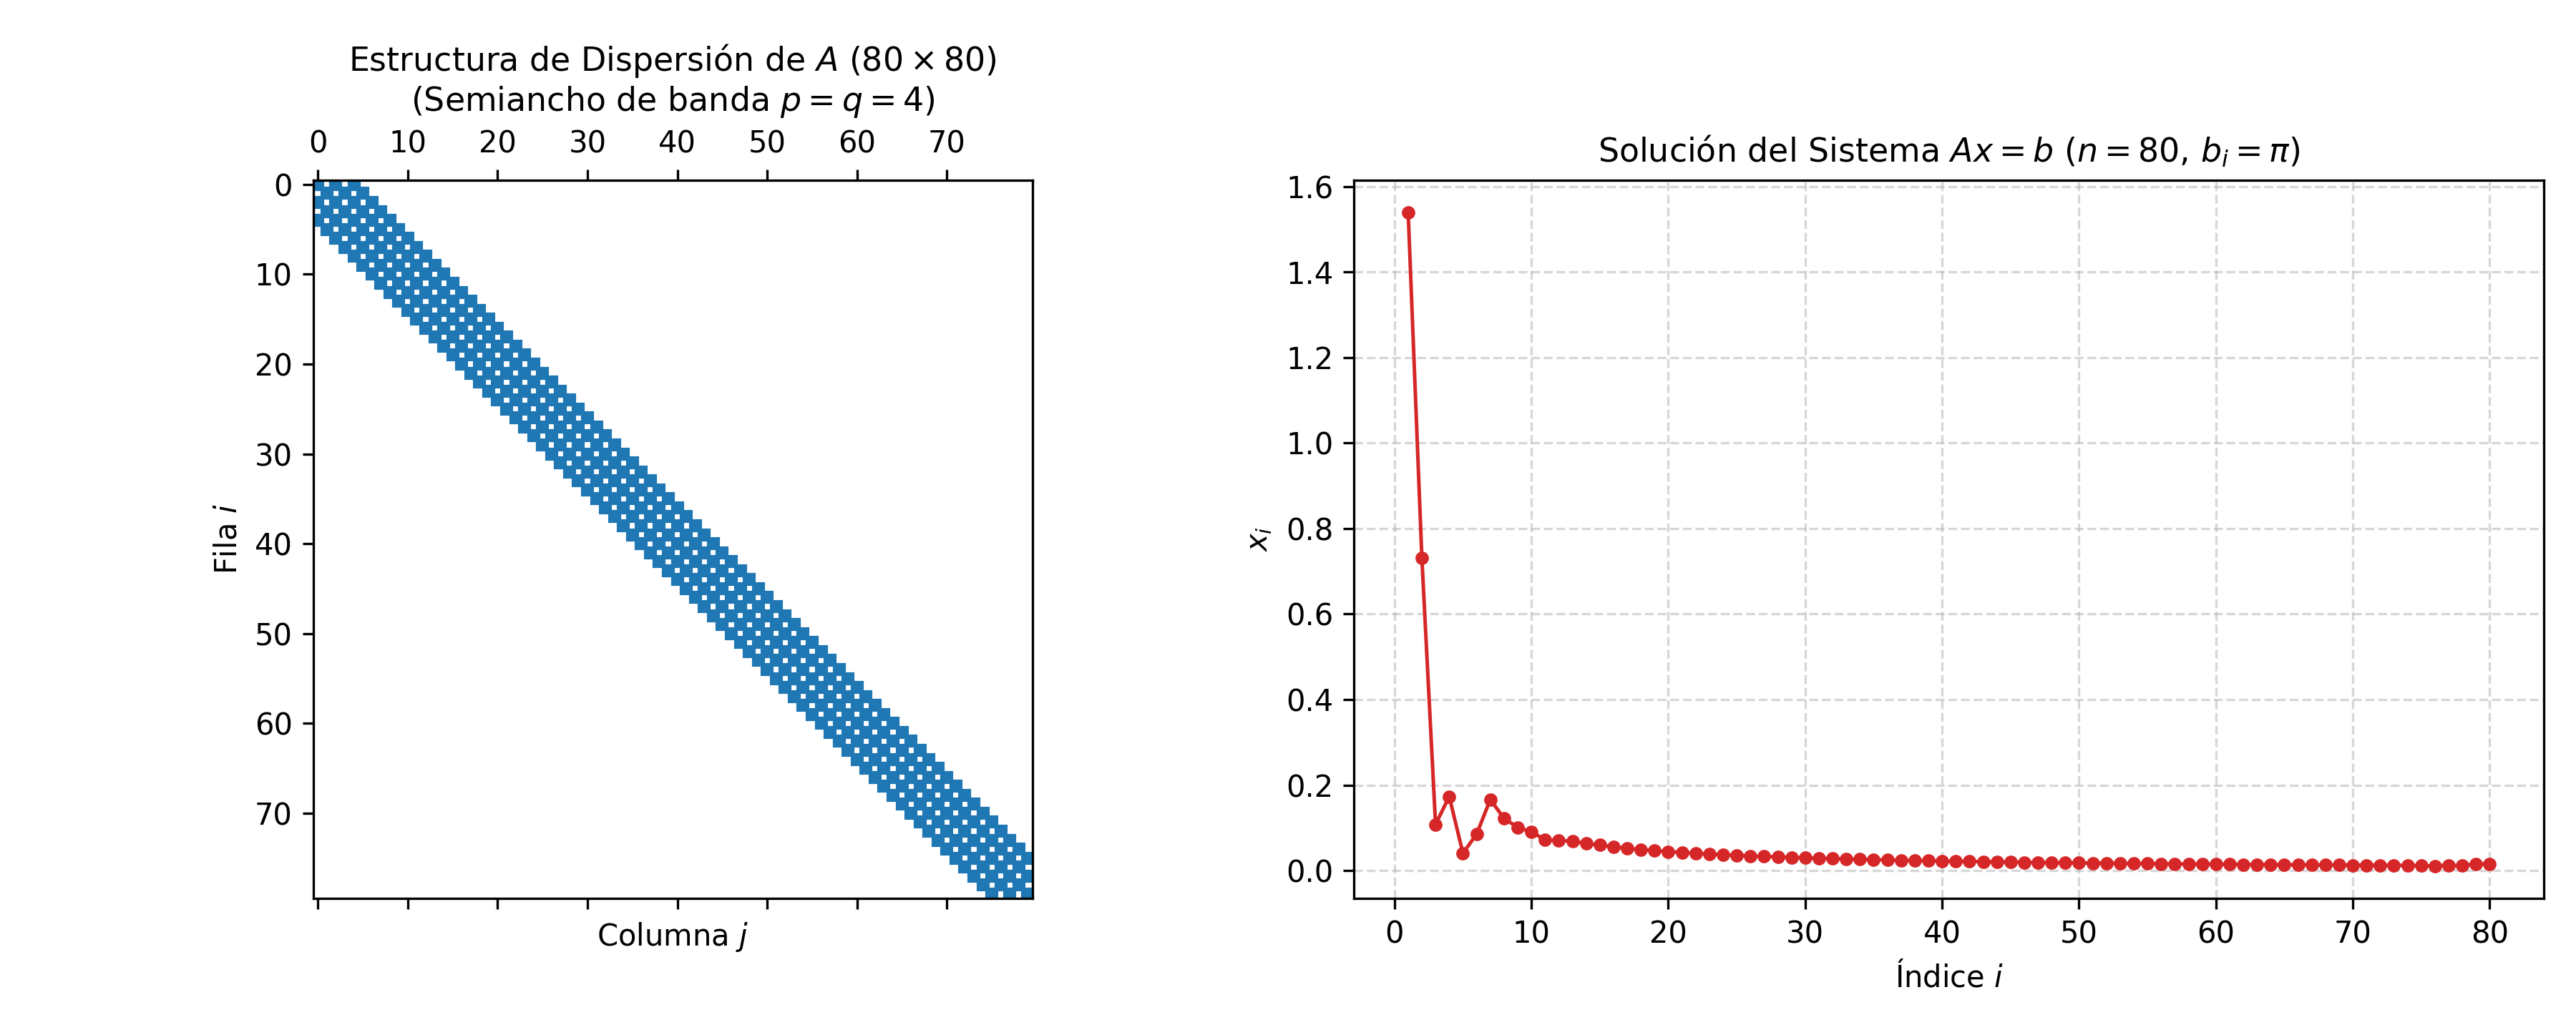
\includegraphics[width=\textwidth]{p3_estructura_y_solucion.png}
    \caption{Patrón de dispersión de la matriz banda $A$ ($80 \times 80$) y perfil del vector solución $x_1, \dots, x_{80}$ para $b_i = \pi$.}
    \label{fig:p3_solucion}
\end{figure}

\begin{figure}[H]
    \centering
    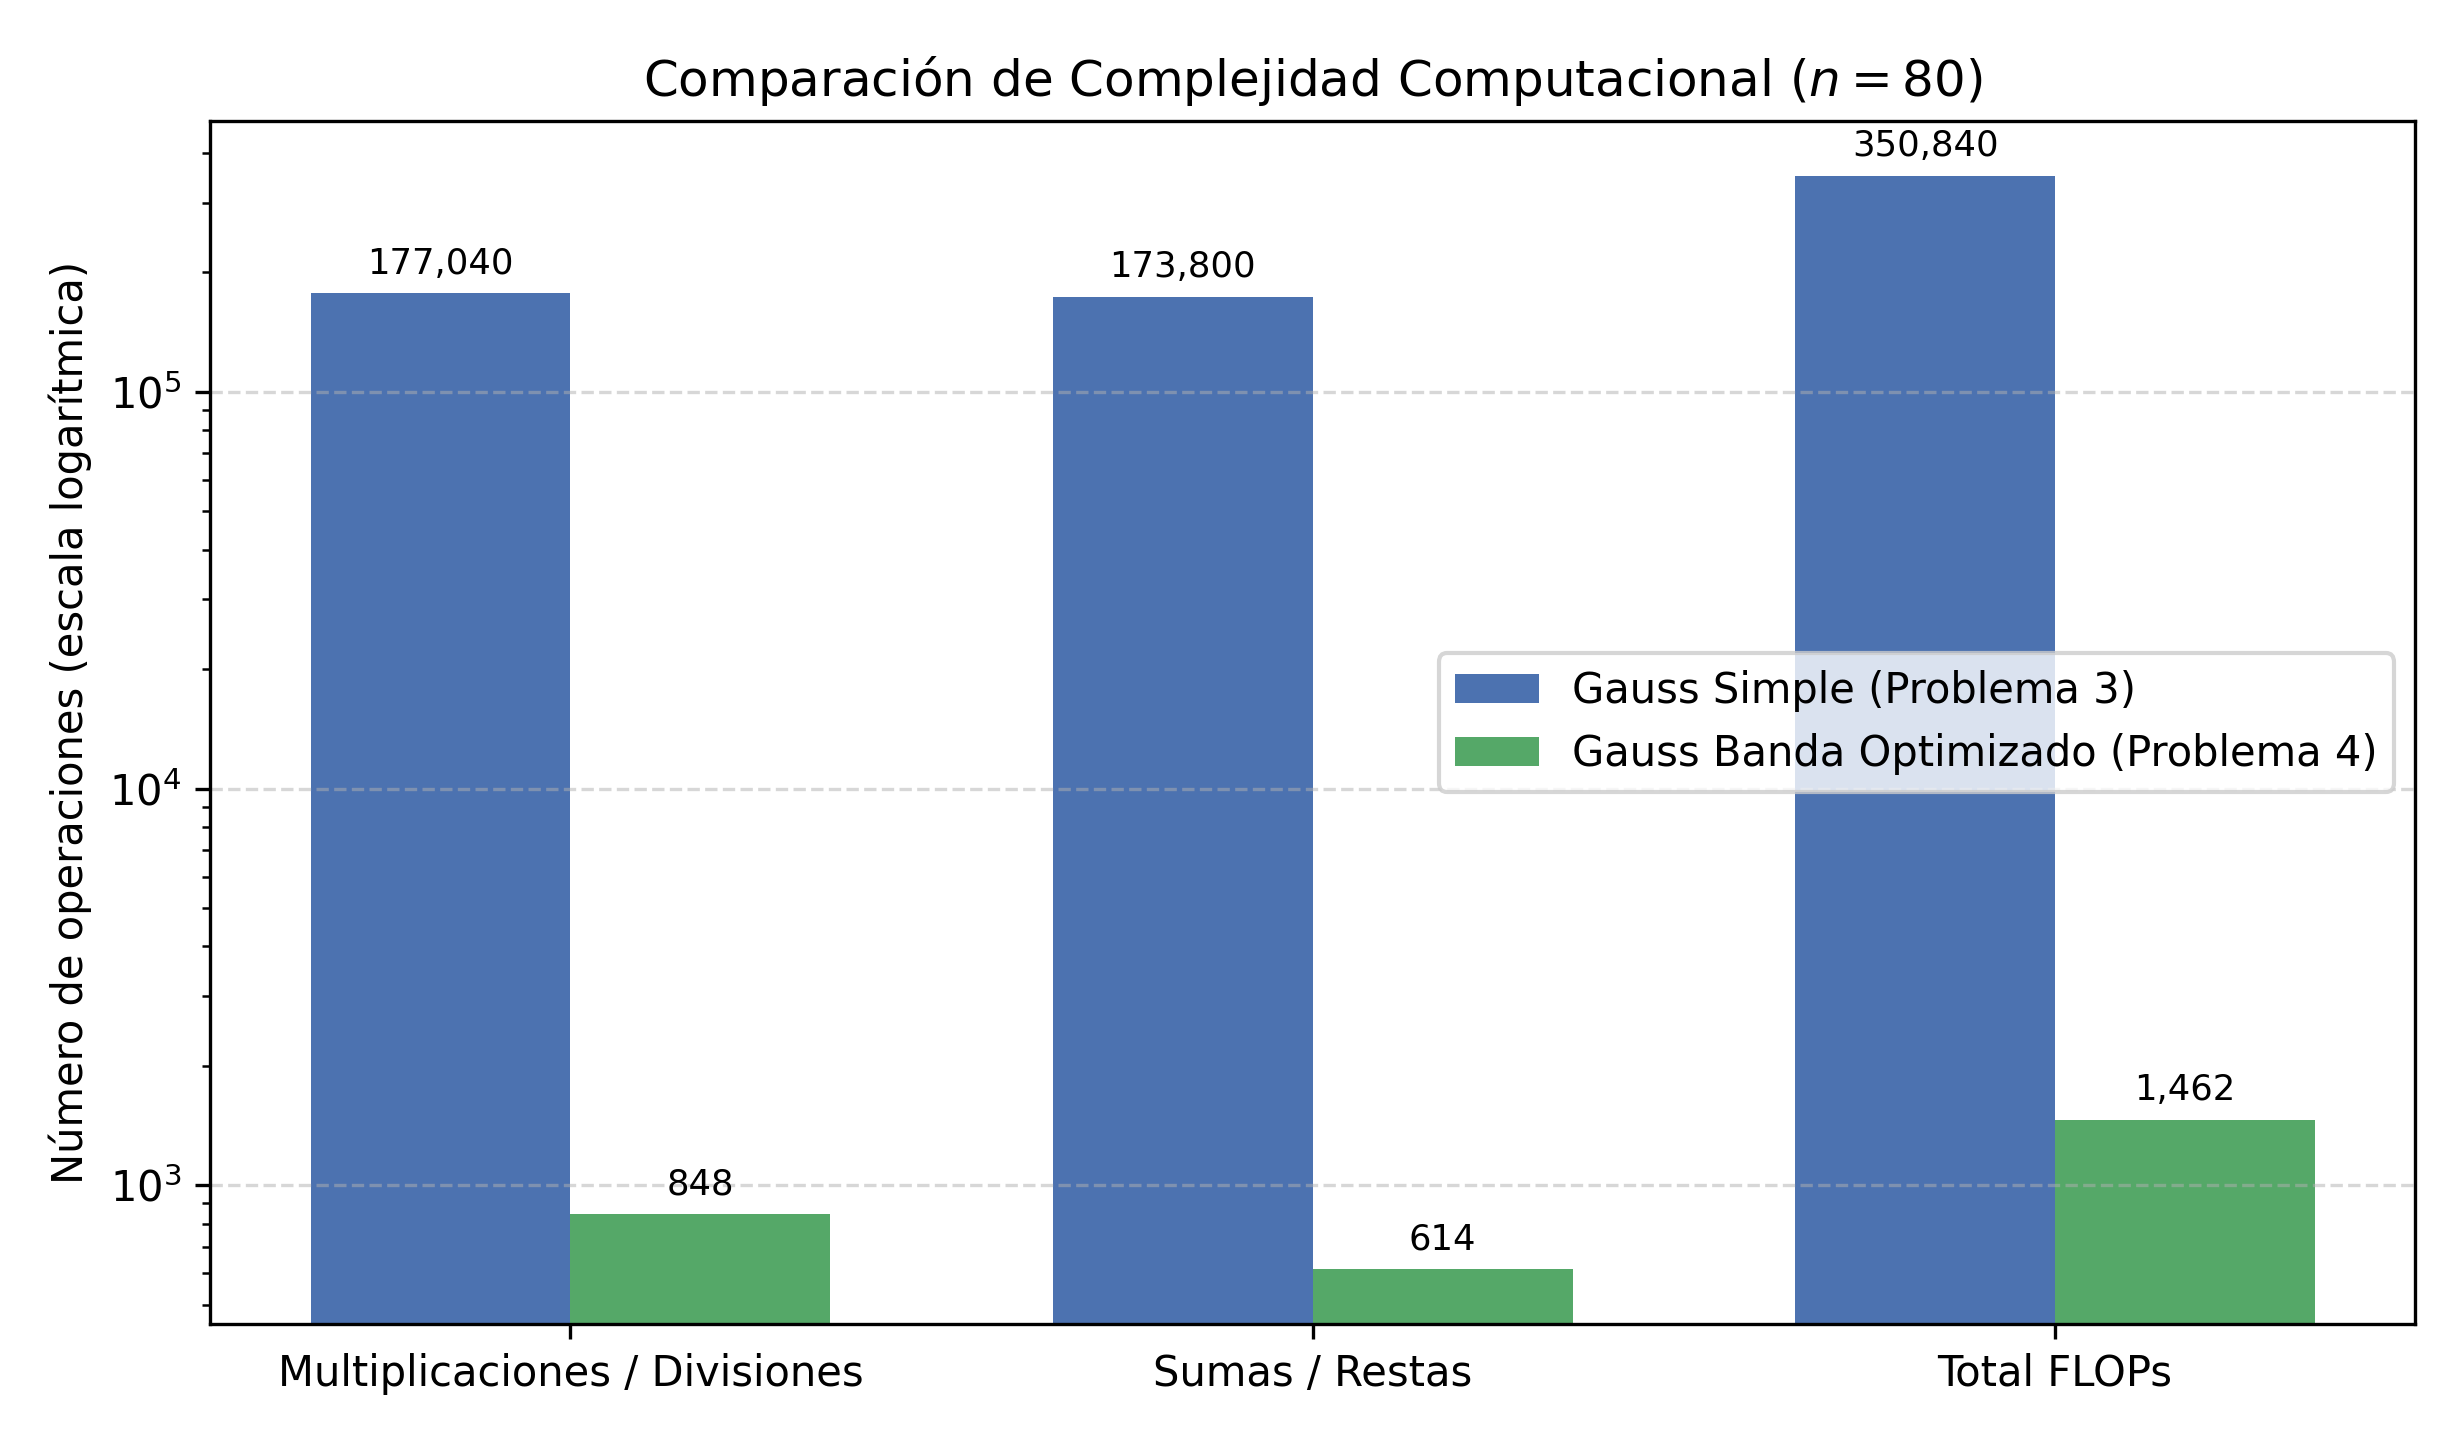
\includegraphics[width=0.84\textwidth]{p4_comparacion_operaciones.png}
    \caption{Comparación en escala logarítmica del número de operaciones aritméticas entre el algoritmo estándar y el algoritmo optimizado para matriz banda.}
    \label{fig:p4_ops}
\end{figure}

\begin{table}[H]
    \centering
    \caption{Vector solución $x = [x_1, x_2, \dots, x_{80}]^T$ del sistema $Ax = b$ ($b_i = \pi$).}
    \label{tab:p3_vector_sol}
    \scriptsize
    \resizebox{\textwidth}{!}{%
    \begin{tabular}{cc|cc|cc|cc}
        \toprule
        $i$ & $x_i$ & $i$ & $x_i$ & $i$ & $x_i$ & $i$ & $x_i$ \\
        \midrule
        $1$  & $1.538734225462$ & $21$ & $0.042465493712$ & $41$ & $0.021848209103$ & $61$ & $0.014700765912$ \\
        $2$  & $0.731421029999$ & $22$ & $0.040534996011$ & $42$ & $0.021330043023$ & $62$ & $0.014464080013$ \\
        $3$  & $0.107970031018$ & $23$ & $0.038769061870$ & $43$ & $0.020835841663$ & $63$ & $0.014234609412$ \\
        $4$  & $0.173284215073$ & $24$ & $0.037178752726$ & $44$ & $0.020363984613$ & $64$ & $0.014012565152$ \\
        $5$  & $0.040556748626$ & $25$ & $0.035705037161$ & $45$ & $0.019912990898$ & $65$ & $0.013802419273$ \\
        $6$  & $0.085248637044$ & $26$ & $0.034347999306$ & $46$ & $0.019481508929$ & $66$ & $0.013593635550$ \\
        $7$  & $0.166448008468$ & $27$ & $0.033092026486$ & $47$ & $0.019068301149$ & $67$ & $0.013384183951$ \\
        $8$  & $0.121979598922$ & $28$ & $0.031919155217$ & $48$ & $0.018672232459$ & $68$ & $0.013187645141$ \\
        $9$  & $0.101249829429$ & $29$ & $0.030826856862$ & $49$ & $0.018292258411$ & $69$ & $0.012971071865$ \\
        $10$ & $0.090457348054$ & $30$ & $0.029807140361$ & $50$ & $0.017927421279$ & $70$ & $0.012785969765$ \\
        $11$ & $0.072028547176$ & $31$ & $0.028852072060$ & $51$ & $0.017576838066$ & $71$ & $0.012702707070$ \\
        $12$ & $0.070263350154$ & $32$ & $0.027956676719$ & $52$ & $0.017239683099$ & $72$ & $0.012526630946$ \\
        $13$ & $0.068754906247$ & $33$ & $0.027115035484$ & $53$ & $0.016915206538$ & $73$ & $0.012376537022$ \\
        $14$ & $0.063243741808$ & $34$ & $0.026322234413$ & $54$ & $0.016602702013$ & $74$ & $0.012209634362$ \\
        $15$ & $0.059711471352$ & $35$ & $0.025574406355$ & $55$ & $0.016301488239$ & $75$ & $0.011290077134$ \\
        $16$ & $0.055708971322$ & $36$ & $0.024867763186$ & $56$ & $0.016011029517$ & $76$ & $0.011141024237$ \\
        $17$ & $0.051874776955$ & $37$ & $0.024199011960$ & $57$ & $0.015730769025$ & $77$ & $0.012173126766$ \\
        $18$ & $0.049245975556$ & $38$ & $0.023565240247$ & $58$ & $0.015460104316$ & $78$ & $0.012017464083$ \\
        $19$ & $0.046778356564$ & $39$ & $0.022963742624$ & $59$ & $0.015198770615$ & $79$ & $0.015428956474$ \\
        $20$ & $0.044483607942$ & $40$ & $0.022392118878$ & $60$ & $0.014945943364$ & $80$ & $0.015237960035$ \\
        \bottomrule
    \end{tabular}%
    }
\end{table}

% ==================== CONCLUSIONES ====================
\section{Conclusiones}
\begin{enumerate}
    \item \textbf{Aritmética finita y condicionamiento (Problema 1):} El truncamiento a $3$ cifras significativas introduce errores iniciales en los coeficientes irracionales que se propagan durante la eliminación. Aunque el pivoteo completo acota todos los multiplicadores ($|m_{ik}| \le 1$), el mal condicionamiento del sistema provoca pérdida de cifras significativas en el último pivote, demostrando que las estrategias de pivoteo controlan el crecimiento algebraico pero no eliminan el error inherente a una precisión de máquina reducida.
    \item \textbf{Costo exacto de inversión matricial (Problema 2):} Aprovechar la estructura dispersa de los vectores canónicos $e^{(p)}$ (omitiendo multiplicaciones por $1$ y sumas con $0$) reduce la complejidad total de calcular $A^{-1}$ a exactamente $n^3$ multiplicaciones/divisiones y $n^3 - 2n^2 + n$ sumas/restas, el equivalente a tres veces el costo cúbico principal de una sola factorización $LU$.
    \item \textbf{Impacto de explotar matrices banda (Problemas 3 y 4):} Acotar los bucles al semiancho de banda $p = q = 4$ y omitir las diagonales impares nulas redujo el conteo de operaciones de $350\,840$ a $1\,462$ FLOPs ($-99.58\%$), preservando exactamente la misma precisión de máquina ($\|Ax - b\|_\infty = 8.88 \times 10^{-16}$) y acelerando la ejecución en más de dos órdenes de magnitud.
\end{enumerate}

\end{document}